\documentclass[10pt,twocolumn]{article}
\usepackage[T1]{fontenc}
\usepackage{lmodern}
\usepackage[utf8]{inputenc}
\usepackage[letterpaper,top=0.75in,bottom=1in,left=0.68in,right=0.68in]{geometry}
\usepackage{setspace}
\usepackage{graphicx}
\usepackage{array}
\usepackage{tabularx}
\usepackage{booktabs}
\usepackage{caption}
\usepackage{enumitem}
\usepackage{hyperref}
\usepackage{soul}
\setlength{\columnsep}{0.17in}
\setlength{\parindent}{0.2in}
\captionsetup{font={small},labelfont=bf}
\sethlcolor{yellow}
\begin{document}
\twocolumn[
  \begin{center}
    {\fontsize{24}{28}\selectfont\textbf{Formato para Presentar Proyectos Modulares (INNI)}\par}\vspace{0.6ex}
    {\fontsize{11}{13}\selectfont Nombre del líder del proyecto, nombre segundo participante, nombre tercer participante, nombre del asesor\par}\vspace{0.8ex}
    {\fontsize{10}{12}\selectfont\itshape CENTRO UNIVERSITARIO DE CIENCIAS EXACTAS E INGENIERÍAS, (CUCEI, UDG)\par}\vspace{0.6ex}
    {\fontsize{9}{11}\selectfont\texttt{johan.herrera4994@alumnos.udg.mx}\par}\vspace{0.3ex}
    {\fontsize{9}{11}\selectfont\texttt{segundo.autor@correo.dom\quad tercer.autor@correo.dom}\par}\vspace{0.3ex}
    {\fontsize{9}{11}\selectfont\texttt{asesor@correo.dom}\par}\vspace{1.0ex}
    {\fontsize{9}{11}\selectfont\texttt{FIRMA DE VISTO BUENO DEL ASESOR}}\par
  \end{center}
  \vspace{1.5ex}
]
\noindent\textbf{\textit{Abstract}}\textbf{---} Este documento es un ejemplo de formato basado en las normas de IEEE para presentar un proyecto modular terminado. Los autores deben seguir las instrucciones, incluyendo formato y tamaño de papel para mantener el estándar de aceptación. Este documento puede interpretarse como un set de instrucciones para presentar su proyecto modular o como una plantilla para hacerlo. Como habrá notado, esta primera sección es para generar un resumen muy corto y a alta escala del alcance del proyecto no deberá utilizar más de 150 palabras en este apartado.

\noindent\textbf{\textit{Palabras claves}}\textbf{ -- }Proyecto modular, formato de registro -- detalles de llenado.

\section*{I. INTRODUCCIÓN}
Este documento es una guía de formato o plantilla. La idea de esta sección es dar una introducción al proyecto modular realizado, de forma concisa y que permita al lector prepararse para los contenidos siguientes.

Debe describir el problema que se va a resolver y su contexto. Se describe a quien va dirigido, es decir el nicho del mercado o la población, la importancia de desarrollar el proyecto.

Beneficios de crear el proyecto, el interés de resolverlo, beneficios, solución y los objetivos de la solución.

\section*{II. TRABAJOS RELACIONADOS}
A partir de esta sección, se desarrollan los contenidos del proyecto modular, de una forma ordenada y secuencial. Nótese que la sección debe ir organizada usando títulos como el anterior para cada tema nuevo incluido. Aparte, se incluyen subtítulos como el siguiente.

\subsection*{A. Subtítulos}
En esta sección se especifican temas detallados que forman parte de un título principal, como el de “Descripción del Desarrollo Del Proyecto Modular”.

\subsection*{B. Especificación del formato del proyecto modular}
El papel debe ser el correspondiente a una hoja carta estilo US, es decir 215.9 mm (8.5\,in) ancho y 279.4 mm (11\,in) largo.

Los márgenes deben ser los siguientes:
\begin{enumerate}[leftmargin=*,label=\arabic*.]
  \item Superior = 19 mm (0.75\,in)
  \item Inferior = 25.4 mm (1\,in)
  \item Izquierdo -- Derecho = 17.3 mm (0.68\,in)
\end{enumerate}

La hoja debe estar dividida en dos columnas, con un espacio de 4.22 mm (0.17\,in) entre columnas.

Si requiere utilizar viñetas, refiérase a la lista de márgenes anterior para ver el estilo.

\section*{III. DESCRIPCIÓN DEL DESARROLLO DEL PROYECTO MODULAR}
Todos los párrafos deben tener indentado o tabulaciones en la primera línea. También, todos los párrafos deben estar alineados de forma justificada y hacia la izquierda.

\subsection*{A. Tipo de letra fuente para el documento}
La totalidad del documento se debe escribir usando Times New Roman o equivalente. Otros tipos de fuente serán utilizados solamente cuando sea requerido para casos especiales.

Los tamaños de fuente se incluyen en la Tabla~\ref{tab:format-sizes}.

\subsection*{B. Título y detalles del autor(es)}
El título debe estar en fuente tamaño 24 puntos. Los nombres de los autores en tamaño de 11 puntos. El nombre de la universidad y departamentos en letra tamaño 10 puntos y cursiva y finalmente los correos electrónicos en tamaño 9 puntos con una fuente tipo Courier.

\begin{table}[t]
  \centering
  \caption{Tamaños de formato de texto}
  \label{tab:format-sizes}
  \begin{tabularx}{\linewidth}{@{}>{\raggedright\arraybackslash}p{0.16\linewidth}*{3}{>{\raggedright\arraybackslash}X}@{}}
    \toprule
    \multicolumn{1}{c}{Tamaño} & \multicolumn{3}{c}{Apariencia (en Times New Roman o Times)} \\
    \cmidrule(l){1-1}\cmidrule(l){2-4}
     & Regular & Negrita & Cursiva \\
    \midrule
    8 & Contenidos de tablas\\Título de figuras\\Referencias a objetos & Negrita & Cursiva \\
    9 & Direcciones de correo electrónico\\(usar fuente Courier)\\Cuerpo del proyecto & Negrita\\Cuerpo del abstract & Cursiva \\
    10 & Subtítulos & Negrita & Cursiva \\
    11 & Nombre del autor & Negrita & Cursiva \\
    24 & Título del proyecto & & \\
    \bottomrule
  \end{tabularx}
\end{table}

El título, autores, universidad y correos deben estar en el encabezado de la primera página, en una sola columna que abarca las dos columnas inferiores. Todo este texto debe estar centrado.

Cada palabra en un título debe iniciar con mayúscula, excepto palabras menores como: “a”, “de”, “y”, “desde” entre otras.

Para evitar confusiones, el apellido de cada autor debe ser escrito siempre.

\subsection*{C. Encabezados de sección}
Cada sección deberá dividirse como máximo en 3 niveles de sub-secciones. Todo subtítulo deberá tener letra de tamaño 10 puntos y cada palabra en el título deberá iniciar con mayúscula excepto las palabras menores como se indicó en la sección II.B.

Observe en la línea anterior cómo se hace una referencia a otra sección del documento, usando el número de título III y el de subtítulo B.

Cuando necesite crear varios niveles de sección en el documento (título, subtítulo, etc.) utilice estas normas:
\begin{enumerate}[leftmargin=*,label=\roman*.]
  \item \textit{Primer nivel}: El primer nivel corresponde al de título, por tanto, debe estar centrado, indexado con números romanos y todas las letras en mayúscula con la primera letra de las palabras mayores en mayor tamaño.
  \item \textit{Segundo nivel}: Un segundo nivel corresponde al subtítulo. Deben estar numerados usando letras seguidas por un punto y alineados a la izquierda. El tipo de letra es de 10 puntos y en cursiva.
  \item \textit{Tercer nivel}: Un tercer nivel es como este que está leyendo. Utiliza letra cursiva de 10 puntos enlistados con números arábigos seguidos por un paréntesis. El cuerpo del ítem debe estar inmediatamente después del encabezado, sin saltos de línea.
\end{enumerate}

\subsection*{D. Figuras y tablas}
Las figuras y tablas deben estar centradas en la columna. Si la figura es muy larga, se puede extender hasta ocupar el espacio de las dos columnas. Cualquier figura o tabla que se extienda más de una columna, pero no ocupe el espacio de las dos columnas, se deberá mostrar centrada en la página y deberá estar siempre en la parte superior o inferior de la página.

Los gráficos deben estar en color, de preferencia utilice colores estándar de manera que puedan ser reproducidos en cualquier sistema. Por colores estándar se entienden rojo, azul, verde, amarillo. Trate de evitar colores complejos como azul claro combinado con azul más fuerte porque podrían confundirse.

Utilice colores sólidos que resalten sobre el fondo de la figura para mejorar el contraste.

Toda figura debe acompañarse de un título en letra de tamaño de 8 puntos, que inicia con la abreviatura “Fig.” para indicar “Figura” y un número de secuencia.

El nombre de la figura debe tener mayúscula solamente en la primera palabra, independientemente de si se trata de una palabra mayor o menor.

El nombre de la figura se utiliza centrado en la columna, o página si la figura se extiende fuera de la columna. Si la descripción se extiende más de una línea, se debe mostrar de forma justificada, como en la Fig.~\ref{fig:solid-colors}.

\begin{figure}[t]
  \centering
  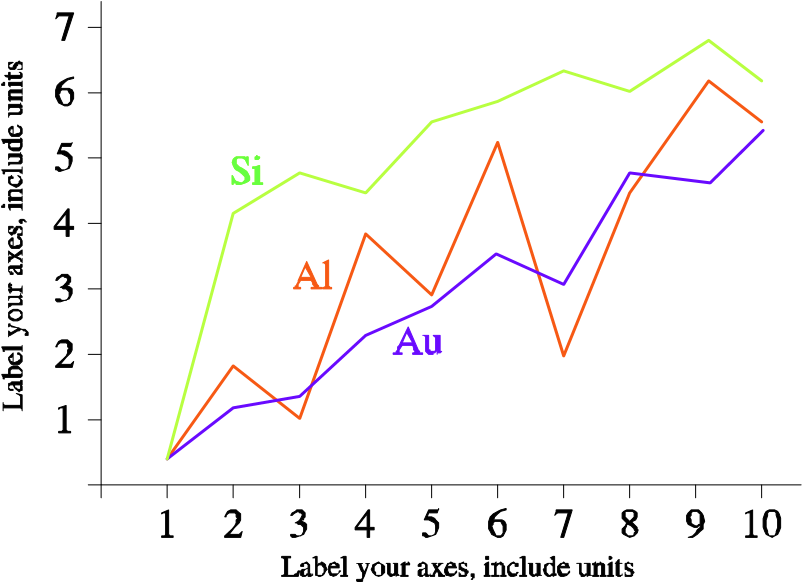
\includegraphics[width=0.75\columnwidth]{img/image3.png}
  \caption{El ejemplo de un gráfico con colores sólidos que resaltan sobre el fondo blanco.}
  \label{fig:solid-colors}
\end{figure}

La Fig.~\ref{fig:low-res} es un ejemplo de una imagen importada al documento. En estos casos, asegúrese de utilizar la resolución adecuada, de manera que la figura se pueda apreciar con claridad en el documento.

No utilice figuras de resolución pobre porque empobrece la calidad del proyecto.

Cuando inserte una figura, asegúrese de verificar lo siguiente:
\begin{itemize}[leftmargin=*]
  \item los colores contrastan adecuadamente,
  \item la imagen es clara,
  \item cualquier texto en la imagen se puede leer claramente.
\end{itemize}

La Fig.~\ref{fig:low-res} muestra un caso donde la resolución no es adecuada, mientras que la Fig.~\ref{fig:good-res} muestra una mejor adaptación de la misma figura.

\begin{figure}[t]
  \centering
  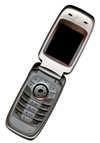
\includegraphics[width=0.55\columnwidth]{img/image1.jpg}
  \caption{Ejemplo de figura con baja resolución}
  \label{fig:low-res}
\end{figure}

\begin{figure}[t]
  \centering
  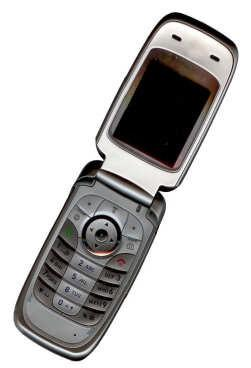
\includegraphics[width=0.53\columnwidth]{img/image2.jpg}
  \caption{Ejemplo de figura con buena resolución}
  \label{fig:good-res}
\end{figure}

\subsection*{E. Títulos de tablas}
Las tablas deben tener un título con letra mayúscula de 8 puntos, centrado en la columna y con letra más grande en el inicio de cada palabra mayor. Antes de la línea del título, se incluye una línea centrada donde se usa la palabra “Tabla” seguida de la numeración de la tabla usando números romanos.

\subsection*{F. Números de página, encabezados y pie de página}
Estos tres elementos no deben ser utilizados.

\subsection*{G. Hiper-vínculos y accesos directos}
Cualquier hiper-vínculo o referencia a Internet debe escribirse por completo. Es decir, escribir el URL completo de la ubicación del recurso en lugar de dejar accesos directos.

Las referencias se escriben usando fuente regular igual que el resto del proyecto.

\subsection*{H. Referencias bibliográficas}
El encabezado de la sección de referencias debe seguir las normas del nivel “título” sin embargo, no debe tener numeración.

Todas las referencias se hacen en letra de 8 puntos.

Utilice cursiva para distinguir los diferentes campos de la referencia. Utilice los ejemplos adjuntos en este documento.

Todas las referencias están numeradas con números arábigos consecutivos que inician en 1 y siempre están encerrados en paréntesis cuadrados (p.e. [1]).

Si en el cuerpo del proyecto hace referencia a alguna de estas referencias, utilice solamente los paréntesis cuadrados y el número correspondiente. Nunca use términos como “ver referencia [4]”, en su lugar use “ver [4]”.

Si son varias referencias juntas, sepárelas con comas.

Las referencias cambian según el tipo de fuente.

Los ejemplos enumerados en la sección de referencias de este documento incluyen:
\begin{enumerate}[leftmargin=*,label=\alph*.)]
  \item ejemplo de un libro [1]
  \item ejemplo de un libro parte de una serie [2]
  \item ejemplo de otro artículo de revista [3]
  \item ejemplo de un artículo de conferencia [4]
  \item ejemplo de una patente [5]
  \item ejemplo de un sitio web [6]
  \item ejemplo de una página de un sitio web [7]
  \item ejemplo de un manual [8]
  \item ejemplo de una hoja de datos [9]
  \item ejemplo de una tesis [10]
  \item ejemplo de un reporte técnico [11]
  \item ejemplo de un estándar [12]
\end{enumerate}

\subsection*{Módulo \hl{Gestión de la tecnología de información}}
\hl{Se describe brevemente la relación que existe de este módulo con el proyecto modular a presentar.}

\subsection*{Módulo \hl{Sistemas robustos, paralelos y distribuidos}}
\hl{Se describe brevemente la relación que existe de este módulo con el proyecto modular a presentar.}

\subsection*{Módulo \hl{Justificación de Cómputo Flexible (softcomputing)}}
\hl{Se describe brevemente la relación que existe de este módulo con el proyecto modular a presentar.}

\section*{IV. RESULTADOS OBTENIDOS DEL PROYECTO}
El propósito de esta sección es resumir los principales resultados discutidos a lo largo del proyecto. Recuerde manejar las conclusiones como enunciados cortos fundamentados en la teoría y los objetivos planteados.

Los resultados deben presentarse en el orden lógico y sucesivo en que fueron encontrados, de forma que sean comprensibles y coherentes.

Los resultados deben describir dos temas claves:

1) Expresar los objetivos reales alcanzados con el proyecto modular al término de su desarrollo.

2) Presentar su relación con la solución planteada.

(Esta sección debe ser escrita utilizando los verbos en pasado)

Esta sección no tiene requisitos especiales de formato.

\section*{V. CONCLUSIONES Y TRABAJO A FUTURO}
El propósito de esta sección es resumir los principales resultados discutidos a lo largo del proyecto. Recuerde manejar las conclusiones como enunciados cortos fundamentados en la teoría y los objetivos planteados.

Esta sección no tiene requisitos especiales de formato.

\section*{RECONOCIMIENTOS}
Esta sección sigue el formato regular del resto del documento. La única observación es notar que el título no está numerado.

En esta sección se agregan agradecimientos a personas que colaboraron en el proyecto pero que no figuran como autores del proyecto.

\section*{REFERENCIAS}
\begin{thebibliography}{12}
  \bibitem{meteveiko} S.~M. Metev and V.~P. Veiko, \textit{Laser Assisted Microtechnology}, 2nd~ed., R.~M. Osgood, Jr., Ed. Berlin, Germany: Springer-Verlag, 1998.
  \bibitem{breckling} J.~Breckling, Ed., \textit{The Analysis of Directional Time Series: Applications to Wind Speed and Direction}, ser. Lecture Notes in Statistics. Berlin, Germany: Springer, 1989, vol.~61.
  \bibitem{zhang} S.~Zhang, C.~Zhu, J.~K.~O. Sin, and P.~K.~T. Mok, “A novel ultrathin elevated channel low-temperature poly-Si TFT,” \textit{IEEE Electron Device Lett.}, vol.~20, pp.~569--571, Nov.~1999.
  \bibitem{wegmuller} M.~Wegmuller, J.~P. von~der Weid, P.~Oberson, and N.~Gisin, “High resolution fiber distributed measurements with coherent OFDR,” in \textit{Proc. ECOC'00}, 2000, paper~11.3.4, p.~109.
  \bibitem{patente} R.~E. Sorace, V.~S. Reinhardt, and S.~A. Vaughn, “High-speed digital-to-RF converter,” U.S. Patent~5\,668\,842, Sept.~16, 1997.
  \bibitem{ieeeweb} (2002) The IEEE website. [Online]. Available: \url{http://www.ieee.org/}
  \bibitem{shell} M.~Shell. (2002) IEEEtran homepage on CTAN. [Online]. Available: \url{http://www.ctan.org/texarchive/macros/latex/contrib/supported/IEEEtran/}
  \bibitem{flexchip} \textit{FLEXChip Signal Processor (MC68175/D)}, Motorola, 1996.
  \bibitem{pdca} “PDCA12-70 data sheet,” Opto Speed SA, Mezzovico, Switzerland.
  \bibitem{karnik} A.~Karnik, “Performance of TCP congestion control with rate feedback: TCP/ABR and rate adaptive TCP/IP,” M.~Eng. thesis, Indian Institute of Science, Bangalore, India, Jan.~1999.
  \bibitem{padhye} J.~Padhye, V.~Firoiu, and D.~Towsley, “A stochastic model of TCP Reno congestion avoidance and control,” Univ. of Massachusetts, Amherst, MA, CMPSCI Tech. Rep.~99-02, 1999.
  \bibitem{ieee80211} \textit{Wireless LAN Medium Access Control (MAC) and Physical Layer (PHY) Specification}, IEEE Std.~802.11, 1997.
\end{thebibliography}
\end{document}
